%This is a LaTeX template for homework assignments
\documentclass{article}
\usepackage[utf8]{inputenc}
\usepackage{amsmath}
\usepackage{amsfonts} 
\usepackage{setspace}
\usepackage{amssymb}
\usepackage{amsmath,bm}
\usepackage{amsthm}
\usepackage{graphicx}
\usepackage{hyperref}
\hypersetup{
    colorlinks=true,
    linkcolor=blue,
    filecolor=magenta,      
    urlcolor=cyan,
    pdftitle={Overleaf Example},
    pdfpagemode=FullScreen,
    }
\urlstyle{same}
\doublespacing
\begin{document}

\section*{Homework 5 Key}
 
\begin{enumerate}%starts the numbering
\item Average value of operator $\hat{p_x^{2022}}$ over PIB of length a.
\\ $ \langle p_x^{2022}\rangle = \int_0^a \psi^*\hat{p_x^{2022}}\psi dx$
\\ $ = \int_0^a \sqrt{\frac{2}{a}}\sin(\frac{\pi n x}{a}) (-i\hbar)^{2022}\frac{\partial^{2022}}{\partial x^{2022}} \sqrt{\frac{2}{a}}\sin(\frac{\pi n x}{a})dx$
\\ $ = -\hbar^{2022}\frac{2}{a}\int_0^a \sin(\frac{\pi n x}{a}) \frac{\partial^{2022}}{\partial x^{2022}} \sin(\frac{\pi n x}{a})dx$
\\The pattern for sin(x) derivatives is 1st cos(x) 2nd -sin(x) 3rd -cos(x) 4th sin(x) and repeat. The 2022nd derivative fits the 2nd derivative pattern.
\\ $ = (\frac{2}{a})(\frac{\pi\hbar n}{a})^{2022}\int_0^a \sin^2(\frac{\pi n x }{a})$
\\ $ = (\frac{\pi\hbar n}{a})^{2022}$

\begin{enumerate}
\item Optional. Find $ \langle e^{\hat{p_x}} \rangle$ if $e^{\hat{p_x}} = \hat{I}+\sum_{k=1}\frac{\hat{p_x^k}}{k!}$ over PIB of length $a$.
\\ $ \langle e^{\hat{p_x}} \rangle = \int_0^a \psi^*(\hat{I}+\sum_{k=1}\frac{\hat{p_x^k}}{k!})$
\\ $ \langle e^{\hat{p_x}} \rangle = \int_0^a \psi^*(1+\sum_{k=1}\frac{(-i\hbar)^k\frac{\partial^k}{\partial x^k}}{k!})$
\\The pattern for sin(x) derivatives is 1st cos(x) 2nd -sin(x) 3rd -cos(x) 4th sin(x) and repeat. When it is an odd derivative, the integral = 0 because odd times even function is odd function. So only even terms are accounted. $(-i)^2=-1$ with 2nd derivative $-sin(x)$ gets positive results. $(-i)^4=1$ with 4th derivative $sin(x)$ gets positive results. All evens terms have
positive numbers.
\\ $= 1 + 0 + \frac{(\pi\hbar n)^2}{2!} + 0 + \frac{(\pi\hbar n)^4}{4!} + 0 + \frac{(\pi\hbar n)^6}{6!} + ... $
\\ models the taylor expansion of $\cosh(\frac{\pi\hbar n}{a}), 1+\frac{x^2}{2!}+\frac{x^4}{4!}+...$
\end{enumerate}

\item Find expectation value for energy for each case. 
\\ Recall that time-independent Schrodinger equation is $\hat{H}\psi=E\psi$ 
\\ $-\frac{\hbar^2}{2m}\frac{d^2\psi(x)}{dx^2}+V(x)\psi(x)=E\psi(x)$
\\ For region II x between 0 and $a$, the potential energy is 0, so the equation becomes:
\\ $-\frac{\hbar^2}{2m}\frac{d^2\psi(x)}{dx^2}=E\psi(x)$, therefore $\hat{H}=-\frac{\hbar^2}{2m}\frac{d^2}{dx^2}$. Hence, to find expectation value, $\langle E\rangle=\frac{\int_0^a \psi^*\hat{H}\psi dx}{\int_0^a \psi^*\psi dx}$.

\begin{enumerate}
\item $\langle E\rangle=\frac{\int_0^a \psi^*\hat{H}\psi dx}{\int_0^a \psi^*\psi dx}$
\\ numerator
\\ $= -\frac{\hbar^2}{2m}\int_0^a (\frac{30}{a-1})^{1/2}\frac{x}{a}(1-\frac{x}{a})\frac{d^2}{dx^2}(\frac{30}{a-1})^{1/2}\frac{x}{a}(1-\frac{x}{a}) dx$
\\ $= -\frac{\hbar^2}{2m}(\frac{30}{a-1}) (-\frac{2}{a^2}) (\frac{1}{a}) \int_0^a x-\frac{x^2}{a} dx$
\\ $= -\frac{\hbar^2}{2m}(\frac{30}{a-1}) (-\frac{2}{a^2}) (\frac{1}{a}) \Big[\frac{x^2}{2}-\frac{x^3}{3a}\Big]_0^a$
\\ $= -\frac{\hbar^2}{2m}(\frac{30}{a-1}) (-\frac{2}{a^2}) (\frac{1}{a}) \frac{a^2}{6}$; 
\\ $= \frac{5\hbar^2}{(a-1)am}$; and $\hbar =\frac{h}{2\pi}$
\\ $= \frac{5h^2}{4\pi^2am(a-1)}$
\\ denominator
\\ $\int_0^a \psi^*\psi dx=\frac{a}{a-1}$
\\divide and get $\frac{5h^2}{4\pi^2a^2m}$
\item $\langle E\rangle=\frac{\int_0^a \psi^*\hat{H}\psi dx}{\int_0^a \psi^*\psi dx}$
\\ $= -\frac{\hbar^2}{2m}\int_0^a (\frac{2}{a+1})^{1/2}\sin(\frac{4\pi x}{a})\frac{d^2}{dx^2}(\frac{2}{a+1})^{1/2}\sin(\frac{4\pi x}{a}) dx$
\\ $= -\frac{\hbar^2}{2m}(\frac{2}{a+1})\int_0^a \sin(\frac{4\pi x}{a})\frac{d^2}{dx^2}\sin(\frac{4\pi x}{a}) dx$
\\ $= -\frac{\hbar^2}{2m}(\frac{2}{a+1})(-\frac{4\pi}{a})^2\int_0^a \sin^2(\frac{4\pi x}{a}) dx$
\\ $= \frac{\hbar^2}{2m}(\frac{2}{a+1})(\frac{16\pi^2}{a^2})(\frac{1}{2}a)$; using trig identity and integrate
\\ $= \frac{2h^2}{ma(a+1)}$; simplify and $\hbar =\frac{h}{2\pi}$
\\ denominator
\\ $\int_0^a \psi^*\psi dx=\frac{a}{a+1}$
\\divide and get $\frac{2h^2}{a^2m}$
\item 
\\ $\langle E\rangle=\frac{n^2h^2}{8ma^2}$ and it was shown in detail in process in 2b where n = energy level within the sin term.
\\ $\psi = (\frac{2}{a})^{1/2}\Big(0.7\sin(\frac{3\pi x}{a})\Big) + (\frac{2}{a})^{1/2}\Big(0.6\sin(\frac{5\pi x}{a})\Big)$
\\ $\langle E\rangle = 0.7\frac{9h^2}{8ma^2} + 0.6\frac{25h^2}{8ma^2}$
\\ Now you have a linear combination of observing energy levels, n=3 and n=5. So you want the probability of observing two states to be equal to one because $\sum |c_k|^2=1$
\\ $0.7^2x+0.6^2x=1$ $x=\frac{100}{85}$
\\ $ 0.7^2x\frac{9h^2}{8ma^2} + 0.6^2x\frac{25h^2}{8ma^2}$
\\ $ \frac{49}{85}\frac{9h^2}{8ma^2} + \frac{36}{85}\frac{25h^2}{8ma^2}$
\end{enumerate}

\item $\pi$ system
    \begin{enumerate}
    \item # of $\pi$ electron = p + 3 
    \\\centerline{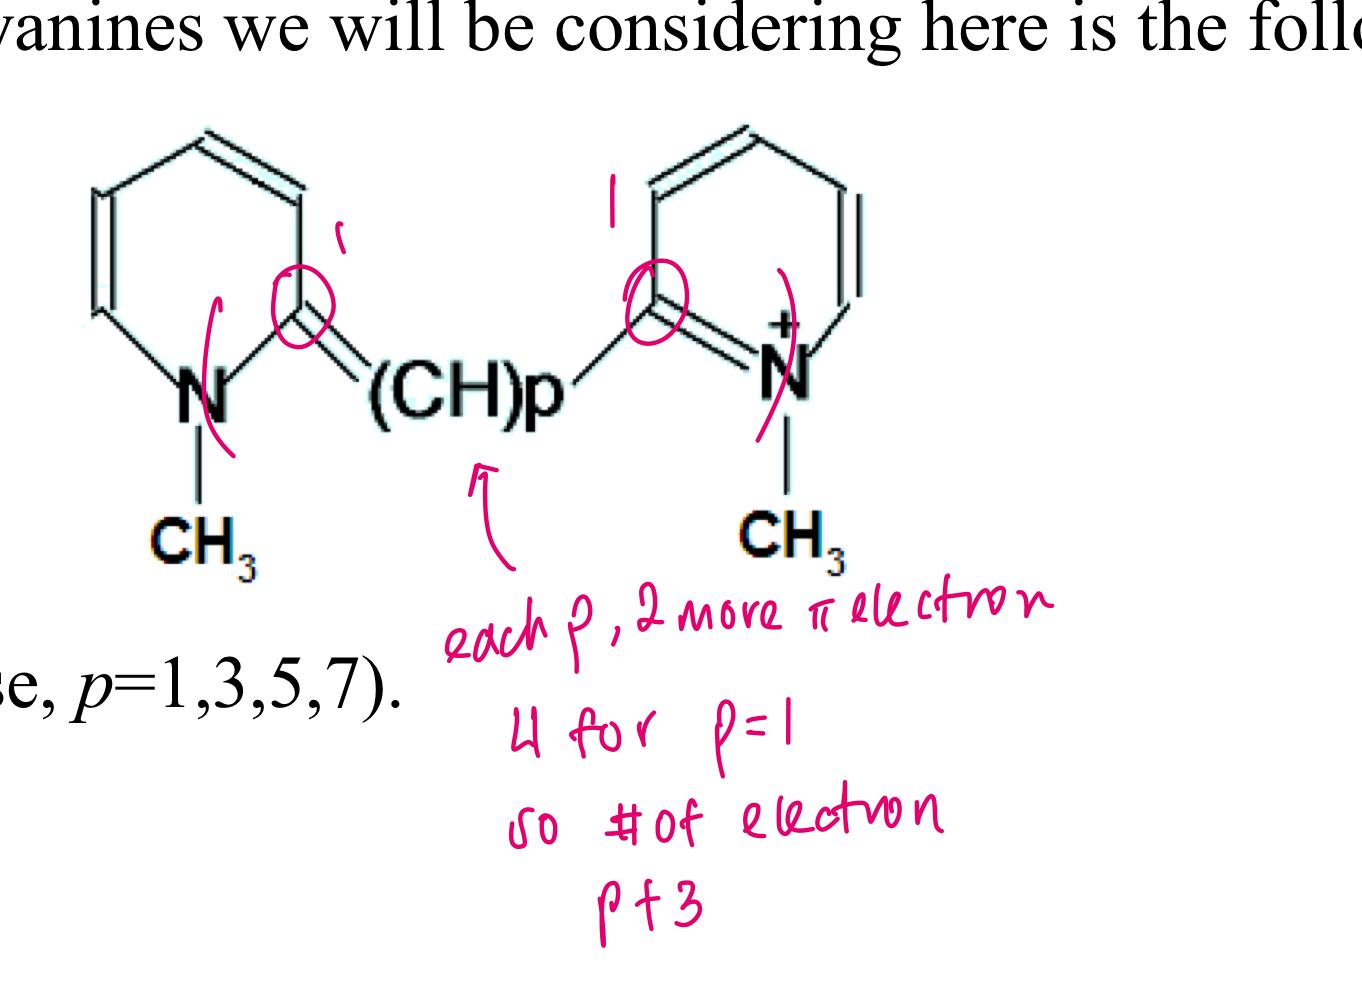
\includegraphics[scale=0.1]{99107.jpg}}
\href{https://www.youtube.com/watch?v=YwoASZrpDoc&t=212s&ab_channel=MichaelEvans}{Click for review on counting pi electrons} 

\item The energy level of a 1D PIB is described as $E=\frac{n^2h^2}{8ma^2}$.
\\To find the energy absorbed from going from HOMO to LUMO:
\\ $\Delta E= E_{LUMO}-E_{HOMO}$
\\ $\Delta E=(n_{LUMO}^2-n_{HOMO}^2)\frac{h^2}{8m_eL^2}$
\\ Two electrons occupy one orbital and we want to find energy associated with exciting one electron so $n=(\frac{N}{2}+1)^2-(\frac{N}{2})^2$. Simplify that and you get $n=N+1$
\\ $\Delta E= (N+1) \frac{h^2}{8m_eL^2}$
\\ $\Delta E= (p+3+1) \frac{h^2}{8m_eL^2}$; plugging in our equation from 3a
\\ $\frac{c}{\lambda}= (p+4) \frac{h}{8m_eL^2}$
\\ $\lambda=\frac{8cm_eL^2}{(p+4)h}$
\\ $\sqrt{\lambda(p+4)}=\sqrt{\frac{8cm_e}{h}}\Big[(p+3)l+a\Big]$
\\ $\frac{\sqrt{\lambda(p+4)}}{\sqrt{\frac{8cm_e}{h}}}=(p+3)l+a$; you can see the $y=mx+b$ format

%For more on figures: https://researchguides.njit.edu/latex/figures#:~:text=Including%20images%20in%20your%20LaTeX,and%20upload%20your%20image%20file.
\\\centerline{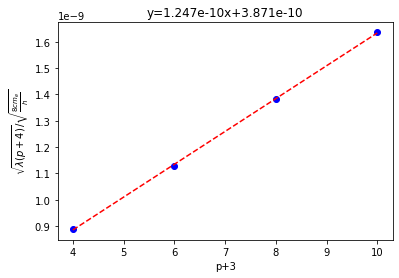
\includegraphics[scale=0.7]{download.png}}
$l=0.1247$ nm
$a=0.3871$ nm

\end{enumerate}
\end{enumerate}%ends the numbering

\end{document}